\documentclass[14pt]{article}
\usepackage{listings}
\usepackage{color}
\usepackage{graphicx}
\usepackage{setspace}

\definecolor{dkgreen}{rgb}{0,0.6,0}
\definecolor{gray}{rgb}{0.5,0.5,0.5}
\definecolor{mauve}{rgb}{0.58,0,0.82}

\lstset{frame=tb,
  language=C,
  aboveskip=3mm,
  belowskip=3mm,
  showstringspaces=false,
  columns=flexible,
  basicstyle={\small\ttfamily},
  numbers=none,
  numberstyle=\tiny\color{gray},
  keywordstyle=\color{blue},
  commentstyle=\color{dkgreen},
  stringstyle=\color{mauve},
  breaklines=true,
  breakatwhitespace=true
  tabsize=3
}







\begin{document}
\title{\huge Topological Sort}
\date{\today}
\maketitle
\begin{center}
\vspace{30 mm}

\title{\huge Student: Marcu Andrei Cristian}
\\\vspace{10 mm}
\title{\huge Computers and Information Technology}
\\\vspace{10 mm}
\title{\huge CE 1.2 A}
\\\vspace{10 mm}
\title{\huge 1st Year}
\date{}
\maketitle

\newpage
\section*{Introduction}
\vspace{20 mm}
Topological sorting for Directed Acyclic Graph (DAG) is a linear ordering of vertices such that for every directed edge uv, vertex u comes before v in the ordering. Topological Sorting for a graph is not possible if the graph is not a DAG.
\\\vspace{10 mm}
A directed acyclic graph (DAG), is a finite directed graph with no directed cycles. 
\\\vspace{10 mm}
Depth-first search (DFS) is an algorithm for traversing or searching tree or graph data structures. The algorithm starts at the root node (selecting some arbitrary node as the root node in the case of a graph) and explores as far as possible along each branch before backtracking.
\\\vspace{10 mm}
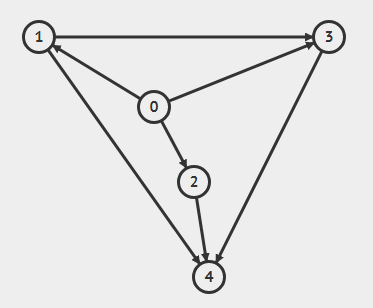
\includegraphics[height=2.5in, width = 2.5in]{graf.png}
\\\vspace{10 mm}
For example DFS in the graph presented above starting from node 0 is : 0, 1, 3, 4, 2. One of the topological sorts of that graph is : 0, 2, 1, 3, 4.
\newpage
\end{center}
\section*{Problem statement}
\\\vspace{5 mm}
Topological sort. Implement two algorithms to determine the topological sort in
directed graphs, e.g., Kosaraju and Tarjan.
\begin{center}
\end{center}
I used two other methods, one with the internal degree of each vertex and the other using DFS.


\newpage
\section*{Pseudocode}
First, we need to generate a random DAG(Directed Acyclic Graph), printing it's adjacency matrix in a file to read it later. After that we can read the matrix and start sorting it, using two methods.
\\
The variables noVertex and noVertexMAX are defined by the user in the header.
\\
Here are the main functions of the program:
\begin{lstlisting}
CheckAcyclic(int Matrix[noVertexMAX][noVertexMAX])
1.  for it1 <- 0 to noVertex-1 do
2.      for it2 <- 0 to noVertex-1 do
3.          aux[it1][it2] <- Matrix[it1][it2]
4.  for it1 <-0 to noVertex-1 do
5.	    visited[it1] <- 0
6.  while count != 0
7.      check <- 0
8.      for it1 <- 0 to noVertex-1 do
9.          internal <- 0
10.         if visited[it1] = 0
11.             for it2 <- 0 to noVertex-1 do
12.                 internal <- internal + aux[it2][it1]
13.             if internal = 0
14.                 check <- 1
15.                 visited[it1] <- 1
16.                 count <- count - 1
17.                 for it2 <- 0 to noVertex-1 do
18.                     aux[it1][it2] <- 0
19.     if check = 0  
20.         return 0
21.  return 1
\end{lstlisting}
\\Now that we have a function that checks if a graph it's acyclic let's generate a graph and test it.
\begin{lstlisting}
randGraph(int Matrix[noVertexMAX][noVertexMAX])
1.  srand(time(0))
2.  for it1 <- 0 to noVertex-1 do
3.      for it2 <- 0 to noVertex do
4.          if it1 = it2
5.              continue
6.          if Matrix[it2][it1] = 0  
7.              Matrix[it1][it2] <- rand() % 2
8.          if CheckAcyclic(Matrix) = 0
9.              Matrix[it1][it2] <- 0
10. for it1 <- 0 to noVertex-1 do
11.     for it2 <- 0 to noVertex-1 do
12.         print Matrix[it1][it2]
13.     print endline
14. print "Number of vertices:",noVertex
\end{lstlisting}
\\ Good, now we have a DAG.Let's start sorting it.Method 1(Internal degree):
\begin{lstlisting}
internal_degree(int Matrix[noVertexMAX][noVertexMAX],int vertex)
1.  sum <- 0
2.  for it1 <- 0 to noVertex-1 do
3.      sum <- sum + Matrix[it1][vertex]
4.  return sum
\end{lstlisting}
\\The function internal\_degree computes the internal degree of a vertex
\begin{lstlisting}
topSort_internal(int Matrix[noVertexMAX][noVertexMAX])
1.  count = 0
2.  for it1 <- 0 to noVertex-1 do
3.      visited[it1] <- 0
4.  while count < noVertex
5.      for it1 <- 0 to noVertex-1 do
6.          if internal_degree(Matrix,it) = 0 and visited[it1] = 0
7.              print it1
8.              visited[it1] <- 1
9.              for it2 <-0 to noVertex-1 do
10.                 Matrix[it1][it2] <- 0
11.             count <- count + 1
\end{lstlisting}
\\Good, now the first topological sort is done, let's see the other one(DFS)
\begin{lstlisting}
noEl_sorted=0
dfs(int it)
1.  visited[it] <- 1
2.  for it1 <- 0 to noVertex-1 do
3.      if Matrix[it][it1] = 1 and visited[it1] = 0
4.          dfs(it1)
5.  sorted[noEl_sorted++] = it
\end{lstlisting}
\\It looks like a basic DFS, which saves the sorted elements in a vector. Well, the magic happens in main, when you read the Matrix by column. If you read the Matrix by column, DFS will do a topological sort instead of his traverse.



\newpage
\section*{Application design}
\vspace{10 mm}
The library contains the header \textbf{\textit{functions.h}} which has all the function prototypes to compute the required operations and all the headers used in the main files.It also contains the defined variables noVertex and noVertexMAX.noVertex=Number of vertices the graph has and noVertexMAX=Number of vertices the graph can have. These are all the functions used:
\\
\\-int CheckAcyclic(int Matrix[noVertexMAX][noVertexMAX]);
\\-void randGraph(int Matrix[noVertexMAX][noVertexMAX]);
\\-int internal\_degree(int Matrix[noVertexMAX][noVertexMAX], int vertex);
\\-void topSort\_internal(int Matrix[noVertexMAX][noVertexMAX]);
\\-void print\_Matrix\_file(int Matrix[noVertexMAX][noVertexMAX]);
\\-void dfs(int it);
\\\vspace{3 mm}
\\The source file \textbf{\textit{main.c}} has all the function calls and some declared functions(CheckAcyclic,randGraph and print\_Matrix\_file).
\\\vspace{3 mm}
Function internal\_degree(int Matrix[noVertexMAX][noVertexMAX], int vertex) computes the internal degree of the vertex
\\\vspace{3 mm}
\\Function topSort\_internal(int Matrix[noVertexMAX][noVertexMAX]) is based on the following idea:
\\Everytime the topological sort starts from the vertex with internal degree 0, this node will be always printed. If we cut all it's edges another vertex will have internal degree 0. We repeat this step until
count(number of elements printed) it's equal to noVertex(number of vertices). We check the internal degree of each vertex using the function internal\_degree
\\\vspace{3 mm}
\\ The adjacency matrix is stored in the file "randMatrix.txt" as a 2D array called 'Matrix'. This array is used by all of our functions. We will use a visited vertices array 'visited', with the value '0' for unvisited and 1 for visited vertices. 
\\\vspace{2 mm}
\\Function DFS(int it) - depth first search works as follows: 
\\1) We visit the starting node and print it
\\2) We visit the nearest unvisited neighbor that can be reached and to the same for that one
\\3) If we exhaust all our options for a node, we return back to the previous node and repeat step 2.
\\\vspace{3 mm}
\\Function CheckAcyclic(int Matrix[noVertexMAX][noVertexMAX] works as follows:\\We generate a matrix aux equal to the original Matrix and a vector visited which is inintially 0. Then we traverse the aux matrix, if the vertex wasn't visited we compute the internal degree. The internal degree should be 0 for the unvisited vertex in order to be acyclic. If the internal degree is 0 we make the boolean variable check 1, the vector visited for this vertex becomes 1 and we cut it's edges. In the end the function returns 1 if the graph is acyclic(check=1) and 0 otherwise.
\\\vspace{2 mm}

Function randGraph(int Matrix[noVertexMAX][noVertexMAX]) generates a random adjacency matrix. srand(time(0)) ensures us that it will be random everytime. If we are on the main diagonal we skip the vertex, if we are elsewhere we generate a random number(0/1) and we check if it makes the graph cyclic. If CheckAcyclic(Matrix) returns 0 then the element generated random before becomes 0 so we can remove the cycle othwerwise we move on. This function also printss the matrix in randMatrix.txt.
\\\vspace{2mm}
Function print\_Matrix\_file(int Matrix[noVertexMAX][noVertexMAX]) prints the matrix from the file.
\\\vspace{3 mm}
\\The main.c file contains the method selector module.If you type 1 it will use the internal degree method, if you type 2 it will use DFS method, and if you type 3 it will use both methods.If the number you type is wrong(!= 1/2/3) it will repeat the action until you insert a right one.

\newpage
\section*{Source Code}
\begin{lstlisting}
//-----------------------------functions.h-------------------------------
#ifndef MAIN_H_INCLUDED
#define MAIN_H_INCLUDED

#include <stdio.h>
#include <stdlib.h>
#include <stdbool.h>
#include <time.h>
#define noVertexMAX 100
#define noVertex 10

int CheckAcyclic(int Matrix[noVertexMAX][noVertexMAX]);
void randGraph(int Matrix[noVertexMAX][noVertexMAX]);
int internal_degree(int Matrix[noVertexMAX][noVertexMAX], int vertex);
void topSort_internal(int Matrix[noVertexMAX][noVertexMAX]);
void print_Matrix_file(int Matrix[noVertexMAX][noVertexMAX]);
void dfs(int it);

#endif



\end{lstlisting}
\begin{lstlisting}
//-----------------------------main.c-------------------------------
#include "functions.h"

int Matrix[noVertexMAX][noVertexMAX];
int sorted[noVertexMAX];
int visited[noVertexMAX];

int main(){
    randGraph(Matrix);

    int it1;
    int it2;
    int MethodSelector=0;

    FILE *randMatrix;
    randMatrix = fopen("randMatrix.txt","r");

    print_Matrix_file(Matrix);
    printf("To use the first method(internal degree method) type 1\n");
    printf("To use the second method(dfs topological sort) type 2\n");
    printf("To use both methods type 3\n");
    printf("Method:");
    scanf("%d",&MethodSelector);
    while(MethodSelector!=1&&MethodSelector!=2&&MethodSelector!=3){
        printf("The number is wrong, please type 1/2/3 to select your method\n");
        printf("Method:");
        scanf("%d",&MethodSelector);
    }
    if(MethodSelector == 1){
        printf("The topological sort using Internal degree method is:");
        for(it1 = 0; it1 < noVertex ; it1++){
            for(it2 = 0 ; it2 < noVertex ; it2++)
                fscanf(randMatrix , "%d" , &Matrix[it1][it2]);
        }
        topSort_internal(Matrix);
    }
    if(MethodSelector == 2){
        printf("The topological sort using DFS method is:");
        for(it1 = 0; it1 < noVertex ; it1++)
            visited[it1] = 0;
        for(it1 = 0; it1 < noVertex ; it1++){
            for(it2 = 0; it2 < noVertex ; it2++)
                fscanf(randMatrix , "%d" , &Matrix[it2][it1]);
        }
        for (it1 = 0; it1 < noVertex; it1++) {
            if (visited[it1] == 0) {
                dfs(it1);
            }
        }
        for (it1 = 0; it1 < noVertex; it1++) {
            printf("%d ",sorted[it1]);
        }
    }
    if(MethodSelector == 3){
        printf("The topological sort using Internal degree method is:");
        for(it1 = 0; it1 < noVertex ; it1++){
            for(it2 = 0; it2 < noVertex ; it2++)
                fscanf(randMatrix,"%d",&Matrix[it1][it2]);
        }
        topSort_internal(Matrix);

        fclose(randMatrix);
        FILE *randMatrix;
        randMatrix = fopen("randMatrix.txt","r"); // Deschidem din nou fisierul pentru a citi matricea pe coloana

        printf("\nThe topological sort using DFS method is:");
        for(it1 = 0; it1 < noVertex ; it1++)
            visited[it1] = 0;
        for(it1 = 0; it1 < noVertex; it1++){
            for(it2 = 0; it2 < noVertex; it2++)
                fscanf(randMatrix,"%d",&Matrix[it2][it1]);
        }
        for (it1 = 0; it1 < noVertex; it1++) {
            if (visited[it1] == 0) {
                dfs(it1);
            }
        }
        for (it1 = 0; it1 < noVertex; it1++) {
            printf("%d ",sorted[it1]);
        }
    }
    fclose(randMatrix);
    return 0;
}
int CheckAcyclic(int Matrix[noVertexMAX][noVertexMAX]){
    int it1;
    int it2;
    int count = noVertex;
    int internal;
    int aux[noVertexMAX][noVertexMAX];
    int visited[noVertexMAX];
    bool check;

    for(it1 = 0; it1 < noVertex; it1++){
        for(it2 = 0; it2 < noVertex; it2++){
            aux[it1][it2] = Matrix[it1][it2];
        }
    }
    for(it1 = 0; it1 < noVertex; it1++)
        visited[it1] = 0;
    while(count != 0){
        check = 0;
        for(it1 = 0; it1 < noVertex; it1++){
            internal = 0;
            if(visited[it1] == 0){
                for(it2 = 0; it2 < noVertex; it2++){
                   internal = internal + aux[it2][it1];
                }
                if(internal == 0){
                    check = 1;
                    visited[it1] = 1;
                    count--;
                    for(it2 = 0; it2 < noVertex; it2++)
                        aux[it1][it2] = 0;
                }
            }

        }
        if(check == 0)
            return 0;
    }
    return 1;
}
void randGraph(int Matrix[noVertexMAX][noVertexMAX]){

    int it1;
    int it2;
    srand(time(0));

    FILE *randMatrix;
    randMatrix = fopen("randMatrix.txt","w");
    //fprintf(randMatrix,"%d \n",noVertex);

    for(it1 = 0; it1 < noVertex; it1++){
        for(it2 = 0; it2 < noVertex; it2++){
            if(it1 == it2){
                continue;
            }
            if(Matrix[it2][it1] == 0){
                Matrix[it1][it2] = rand() % 2;
            }
            if(CheckAcyclic(Matrix) == 0){
                Matrix[it1][it2] = 0;
            }
        }
    }
    for(it1 = 0; it1 < noVertex; it1++){
        for(it2 = 0; it2 < noVertex; it2++){
            fprintf(randMatrix , "%d " , Matrix[it1][it2]);
        }
        fprintf(randMatrix , "\n");
    }
    fprintf(randMatrix , "Number of vertices:%d" , noVertex);
    fclose(randMatrix);
}
void print_Matrix_file(int Matrix[noVertexMAX][noVertexMAX]){
    int it1;
    int it2;
    FILE *randMatrix;
    randMatrix = fopen("randMatrix.txt","r");

    printf("The adjacency matrix of the random directed acyclic graph is:\n");
    for(it1 = 0 ; it1 < noVertex ; it1++){
        for(it2 = 0 ; it2 < noVertex ; it2++)
            printf("%d " , Matrix[it1][it2]);
        printf("\n");
    }
    fclose(randMatrix);
}
\end{lstlisting}
\begin{lstlisting}
//-----------------------------topSortDFS.c-------------------------------
#include "functions.h"

int Matrix[noVertexMAX][noVertexMAX];
int sorted[noVertexMAX];
int visited[noVertexMAX];
int noEl_sorted=0;

void dfs(int it) {
    int it1;
    visited[it] = 1;
    for (it1 = 0; it1 < noVertex; it1++) {
        if (Matrix[it][it1] == 1 && visited[it1] == 0){
            dfs(it1);
        }
    }
    sorted[noEl_sorted++] = it;
}


\end{lstlisting}
\begin{lstlisting}
//-----------------------------topSortInternal.c-------------------------------
#include "functions.h"

int internal_degree(int Matrix[noVertexMAX][noVertexMAX],int vertex){
    int it1;
    int sum=0;
    for(it1=0;it1<noVertex;it1++){
        sum=sum+Matrix[it1][vertex];
    }
    return sum;
}
void topSort_internal(int Matrix[noVertexMAX][noVertexMAX]){
    int it1;
    int it2;
    int visited[noVertexMAX];
    int count=0;

    for(it1=0;it1<noVertex;it1++)
        visited[it1]=0;
    while(count<noVertex){
        for(it1=0;it1<noVertex;it1++)
            if(internal_degree(Matrix,it1)==0&&visited[it1]==0){
                printf("%d ",(it1));
                visited[it1]=1;
                for(it2=0;it2<noVertex;it2++)
                    Matrix[it1][it2]=0;
                count++;
            }
    }
}
\end{lstlisting}
\section*{Experiments and results}
Example with first method   \\
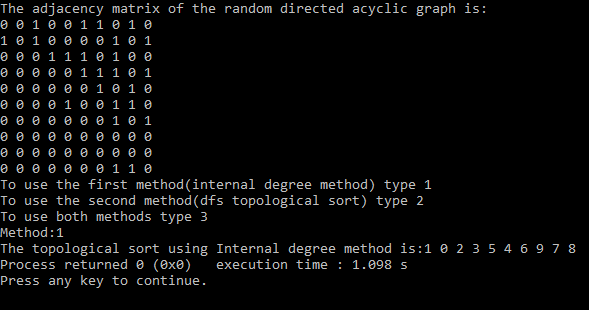
\includegraphics[height=3.1in, width = 4in]{exemplu1.png}\\
Example with second method  \\
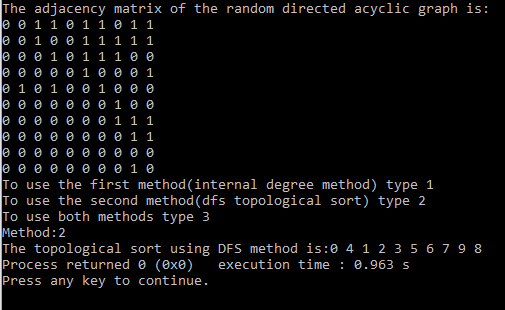
\includegraphics[height=3.1in, width = 4in]{exemplu2.png}\\
Example with both methods  \\
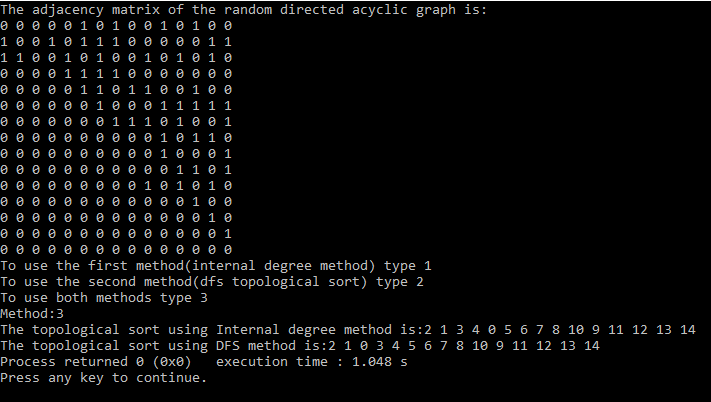
\includegraphics[height=3.1in, width = 4in]{exemplu3.png}


\newpage
\section*{Conclusions}
\vspace{20 mm}
Working on this problem, I have acquired lots of knowledge about graphs, topological sort and also about writing code, to make it more understable, to create makefiles and headers. Also I've filled my lacks of knowledge about GitHub
\\\vspace{20mm}
\section*{References}
\large www.stackoverflow.com
\\
\\\vspace{6mm}
\\
https://www.geeksforgeeks.org/
\\
\\\vspace{6mm}
\\
https://visualgo.net/en/dfsbfs
\\
\\\vspace{6mm}
\\
http://www.cplusplus.com/
\\
\\\vspace{6mm}
\\
http://www.sharelatex.com

\end{document}
